\documentclass[11pt,aspectratio=169]{beamer}
\usetheme{default}
\usepackage[utf8]{inputenc}
\usepackage[T1]{fontenc}
\usepackage{hyperref}
\usepackage{multimedia}
\usepackage{animate}
\usepackage{xmpmulti}
\usepackage{media9}
\usepackage{subfig}
% \usepackage[font=small]{caption}
% \usepackage[font=small]{subcaption}

\usepackage[tensorialbold]{mescommandes}
\usepackage[babel=true,kerning=true]{microtype}
\usepackage{amsmath}
\usepackage{amsfonts}
\usepackage{amssymb}
\usepackage{mathrsfs}
\usepackage{graphicx}
\graphicspath{{figures/}}
\usepackage{fancybox}
\usepackage{textcomp}
\usepackage{multicol}
\usepackage{xcolor}
\usepackage{lmodern}
\RequirePackage{tikz}
\usetikzlibrary{patterns} 
%\usepackage[hang,tight,scriptsize]{subfigure}
\usetikzlibrary{shapes}
\usetikzlibrary{snakes}
\usepackage{pgfplots}
%\usepackage{pgfplotsthemetol}
\pgfplotsset{compat=newest,
	grid=both,
        tick label style={font=\normalsize},
	label style={font=\normalsize},
	legend style={font=\normalsize},
	legend cell align={left},
        yticklabel style={/pgf/number format/fixed},
        % define user colormap
	colormap={tol}{[1cm] rgb255(0cm)=(120,28,129) rgb255(1cm)=(63,96,174) rgb255(2cm)=(83,158,182) rgb255(3cm)=(109,179,136) rgb255(4cm)=(202,184,67) rgb255(5cm)=(231,133,50) rgb255(6cm)=(217,33,32)}
}

% define user color
\definecolor{col1}{RGB}{51,34,136}
\definecolor{col2}{RGB}{136,204,238}
\definecolor{col3}{RGB}{17,119,51}
\definecolor{col4}{RGB}{221,204,119}
\definecolor{col4}{RGB}{204,102,119}
\definecolor{col5}{RGB}{217,33,32}
\definecolor{col6}{RGB}{170,68,153}
\definecolor{col7}{RGB}{227,156,55}

%% User colors
\definecolor{Purple}{RGB}{120,28,129}
\definecolor{Blue}{RGB}{63,96,174}
\definecolor{Duck}{RGB}{83,158,182}
\definecolor{Green}{RGB}{109,179,136}
\definecolor{Yellow}{RGB}{202,184,67}
\definecolor{Orange}{RGB}{231,133,50}
\definecolor{Red}{RGB}{217,33,32}

%\setcounter{tocdepth}{1}
\usefonttheme{professionalfonts}
%\usetheme[progressbar=foot,subsectionpage=progressbar,sectionpage=none]{metropolis}
\usetheme[progressbar=foot,subsectionpage=none,sectionpage=progressbar]{metropolis}
\useoutertheme{Headinfoline}
\setbeamertemplate{section in toc}{{\inserttocsectionnumber.}~\inserttocsection    \vspace{-.05\baselineskip}}
% \setbeamertemplate{subsection in toc}{{\inserttocsubsectionnumber.}~\inserttocsubsection    \vspace{-.1\baselineskip}}

\setbeamerfont{section in toc}{size=\normalsize,series=\bfseries}
\setbeamerfont{subsection in toc}{size=\footnotesize}
    
%% CHANGE COLOR SETTINGS
\definecolor{mDarkBrown}{HTML}{604c38}
\definecolor{mDarkTeal}{HTML}{23373b}
\definecolor{mLightBrown}{HTML}{EB811B}
\definecolor{mLightGreen}{HTML}{14B03D}
\definecolor{CNBlue}{RGB}{16,38,72}
\definecolor{CNYellow}{RGB}{250,182,0}

%% fg= ; bg= background 
\setbeamercolor{normal text}{ fg= CNBlue!90 , bg= black!2 }
%\setbeamercolor{alerted text}{ fg=mDarkTeal  }
%\setbeamercolor{exemple text}{ fg=mDarkTeal  }





\setbeamerfont{bibliography entry author}{size=\scriptsize,series=\normalfont}
\setbeamerfont{bibliography entry title}{size=\scriptsize,series=\bfseries}
\setbeamerfont{bibliography entry location}{size=\scriptsize, series=\normalfont}
\setbeamerfont{standout}{size=\Large,series=\bfseries}
%%%%%%%%%%caracterisation du document %---------------------------------------------------------------------
\hypersetup{
	pdftitle    = {Formulation of the DGMPM},
	pdfsubject  = {MS team meeting - March 2018},
	linkcolor    = red,
	pdfauthor   = {Adrien Renaud},
	pdfkeywords = {numerical simulation, hyperbolic problems, discontinuous Galerkin}
	colorlinks=true,
	linkcolor=black,
	citecolor=blue,
	urlcolor=blue
}



%%-------------- Construction de la page de presentation -------------------------------------------------------
\title[The Discontinuous Galerkin Material Point Method]
{\Large\bf  {The Discontinuous Galerkin Material Point Method: \\application to hyperbolic problems in solid mechanics}}

\date[]{
	\footnotesize{PhD defense} --
	December 14 2018 \\ \hspace*{7.cm}\includegraphics[trim = 0cm 4cm 0cm 0cm, clip,scale=0.1]{Logo_GEM.pdf} \hspace*{2.cm}\includegraphics[scale=0.25]{Logo_ECN.pdf}}%\logo{ \includegraphics[trim = 0cm 4cm 0cm 0cm, clip,scale=0.1]{Logo_GEM.pdf} \hspace*{2.cm}\includegraphics[scale=0.25]{Logo_ECN.pdf}}
\author{A. Renaud \\ Supervisors: T. Heuz\'e, L. Stainier} 


%------------------------------------------------------------------------

\setbeamertemplate{bibliography item}{\insertbiblabel}


%% Baptist's beamer clock
\newcommand{\myBeamerClock}[2]{
  % #1 is the radius of the clock
  % #2 is the vertical shift for inline placement
  \tikz[baseline=#2]{
    \filldraw (0,0) -- (0,#1) arc (90:(90-\insertframenumber/(\inserttotalframenumber)*360):#1);
    \draw (0,0) circle (#1);
  }
}


\begin{document}
\begin{frame}[plain]
  \maketitle
\end{frame}

\begin{frame}[plain]{Outline}
  \tableofcontents[hideallsubsections]
\end{frame}



% \begin{frame}[plain]{Outline}
%   \begin{columns}
%     \begin{column}{0.5\textwidth}
%       \tableofcontents%[hideallsubsections]
%     \end{column}
%     \begin{column}{0.5\textwidth}
%       \tableofcontents%[hideallsubsections]
%     \end{column}
%   \end{columns}
% \end{frame}


\section{Motivations}

\begin{frame}{From physics to the mathematical model}
  % Concerned with solid dynamics problems such as Impact or crash-proof design.
  % in the first case, one wants to ensure that a structure undegoing dynamic loadings remains usable while in the latter, it is expected to dissipate as much energy as possible so that the passengers are safe
  
  % On the other hand, high-speed forming techniques such as electromagnetic forming also involve dynamic loadings

  % At last, another challenging field of dynamics is the reliability of structures to earthquakes
  % Here is depicted the mass damper of the Taipei 101 tower which design was possible thanks to a good understanding of the physics.
  \vspace{-0.6cm}
  \begin{overprint}
    \onslide<1>
    \begin{columns}
      \begin{column}{0.45\textwidth}
        \begin{block}{Solid dynamics problems}
          \begin{itemize}
          \item[] \textbf{Impact; Crash-proof design}
          \item[] High-speed forming
          \item[] Earthquake reliability of structures 
          \end{itemize}
        \end{block}
      \end{column}
      
      \begin{column}{0.55\textwidth}
      \end{column}
    \end{columns}
    
    \begin{figure}[ht]
      \centering
      \subcaptionbox{Bird strike on aircrafts}{\includegraphics[height=0.3\paperheight]{section1/pictures/birdstrike.jpg}}
      \subcaptionbox{Glasgow Museum of Transport}{\includegraphics[height=0.3\paperheight]{section1/pictures/crash2.jpg}}
    \end{figure}
    
    \onslide<2>
    \begin{columns}
      \begin{column}{0.45\textwidth}
        \begin{block}{Solid dynamics problems}
          \begin{itemize}
          \item[] Impact; Crash-proof design
          \item[] \textbf{High-speed forming}
          \item[] Earthquake reliability of structures 
          \end{itemize}
        \end{block}
      \end{column}
      
      \begin{column}{0.55\textwidth}
      \end{column}
    \end{columns}
    \centering
      \movie[height = 0.35\paperheight,width=0.25\linewidth,loop,poster,autostart]{}{%
      section1/animation/output3.mp4}\\
    \scriptsize Electromagnetic forming \cite{Guillaume}
    \footnoteCite{Guillaume}
    
    \onslide<3>
    \begin{columns}
      \begin{column}{0.45\textwidth}
        \begin{block}{Solid dynamics problems}
          \begin{itemize}
          \item[] Impact; Crash-proof design
          \item[] High-speed forming
          \item[] \textbf{Earthquake reliability of structures}
          \end{itemize}
        \end{block}
      \end{column}
      
      \begin{column}{0.55\textwidth}
      \end{column}
    \end{columns}

    \centering
    \includegraphics[scale=0.15]{section1/pictures/TaipeiTower.png} \quad
    \includegraphics[scale=0.08]{section1/pictures/MassDamper.jpg}\\
    \scriptsize Taipei 101 mass damper

    \onslide<4>
    \begin{columns}
      \begin{column}{0.45\textwidth}
        \begin{block}{Solid dynamics problems}
          \begin{itemize}
          \item[] Impact; Crash-proof design
          \item[] High-speed forming
          \item[] Earthquake reliability of structures 
          \end{itemize}
        \end{block}
      \end{column}
      
      %% The governing equations allowing to mathematically model those physical phenomena are composed of Conservation laws and constitutive equations, which can be written as a hyperbolic system
      %% Even though models can be built, the complex geometries, waves propagating in solids and the possibly finite deformations make in general the exact solution not possible.
      %% As a result, the numerical simulation based on space and time approximations becomes helpfull
      \begin{column}{0.55\textwidth}
        \begin{block}{Partial differential equations}
          \begin{equation*}
            \Rightarrow \left\lvert
              \begin{aligned}
                & \text{Conservation laws} \\
                & \text{Constitutive equations} 
              \end{aligned}
            \right. = \textbf{Hyperbolic system}
            % Préciser les équations dans le dévelopement de la DGMPM
          \end{equation*}
        \end{block}
      \end{column}
    \end{columns}
    
    \begin{block}{Difficulties for the solution of hyperbolic equations:}
      \begin{itemize}
      \item complex geometries
      \item waves propagating/interacting in solids \cite{Wang}
      \item finite deformations
      \end{itemize}
    \end{block}
    \textbf{$\Rightarrow$ Resort to numerical simulation:} space and time discretization techniques
    \footnoteCite{Wang}
  \end{overprint}
  
\end{frame}

\begin{frame}{Suitability of some explicit methods}
  %% Among the big stars of existing numerical methods, the FEM
  \begin{block}{The Finite Element Method \cite{Belytschko}}
    \vskip 4pt
    \begin{overprint}
      \onslide<1>
      \begin{columns}
        \begin{footnotesize}
          \begin{column}{0.5\textwidth}
            \begin{itemize}
            \item[] Mesh-based space discretization
            \item[] Weak form of balance equation
            \end{itemize}
          \end{column}
          \begin{column}{0.5\textwidth} 
            \begin{itemize}
            \item[] Polynomial approximation
            \item[] Gauss points constitutive update
            \end{itemize}
          \end{column}
        \end{footnotesize}
      \end{columns}
      \onslide<2>
      \begin{columns}
        \begin{footnotesize}
          \begin{column}{0.5\textwidth}
            \begin{itemize}
            \item[] Mesh-based space discretization
            \item[] Weak form of balance equation
            \end{itemize}
          \end{column}
          \begin{column}{0.5\textwidth} 
            \begin{itemize}
            \item[] Polynomial approximation
            \item[] Gauss points constitutive update
            \end{itemize}
          \end{column}
        \end{footnotesize}
      \end{columns}
      \vskip -10pt
      \begin{columns}
        \begin{column}{0.48\textwidth}
          \begin{block}{\footnotesize Lagrangian formulation}
            \centering
            \begin{tikzpicture}[scale=0.4]
              \tkzKiviatDiagram[lattice=4,
              label style/.append style={font=\tiny},radial  style/.style ={->},lattice style/.style ={white,opacity=0}]{CFL,Non-diffusive,Mesh robustness,Non-oscillating,High-order}
              \tkzKiviatLine[thick,color = black!50](4,4,4,4,4)
              
              \tkzKiviatLine[thick,color = Blue,fill= Blue,opacity=.7](4,4,1,1,3)
            \end{tikzpicture}
          \end{block}
        \end{column}
        \begin{column}{0.48\textwidth}
          % \begin{block}{\footnotesize Eulerian formulation}
          %   \centering
          %   \begin{tikzpicture}[scale=0.4]
          %     \tkzKiviatDiagram[lattice=4,
          %     label style/.append style={font=\tiny},radial  style/.style ={->},lattice style/.style ={white,opacity=0}]{CFL,Non-diffusive,Distortion-free,Non-oscillating,High-order}
          %     \tkzKiviatLine[thick,color = black!50](4,4,4,4,4)
              
          %     \tkzKiviatLine[thick,color = Blue,fill= Blue,opacity=.7](4,2,4,1,3)
          %   \end{tikzpicture}
          % \end{block}
        \end{column}
      \end{columns}
    \end{overprint}
  \end{block}
\footnoteCite{Belytschko}
\end{frame}

%% Pas forcément mettre en avant le tangling
%% Approches Lagrangiennes FVM qui ont des di
%% Citer Maire le papier de 2006 sur la définition de la vitesse nodale (similaire au DG puisque v est discontinue) -> pas tant mesh entanglement que mesh update issues (le second étant valable même en total lagrangian)
%% Virer l'Eulérien; mettre mesh drawbacks; citer le cas échéant; et préciser à l'oral les mesh drawbacks: pour FVM, il s'agit de bouger le maillage avec un champ de vitesse discontinu
\begin{frame}{Suitability of some explicit methods}
  \begin{block}{The Finite Volume Method \cite{Leveque}}%\cite{Haider_FVM} for total Lagrangian
    \vspace{-0.2cm}
    \begin{overprint}
      \onslide<1>
      \vspace{-0.2cm}
      \begin{columns}
        \begin{footnotesize}
          \begin{column}{0.4\textwidth}
            \begin{itemize}
            \item[] Mesh-based space discretization
            \item[] Conservation laws
            \end{itemize}
        \end{column}
        \begin{column}{0.6\textwidth}
            \begin{itemize}
            \item[] Cell-wise approximation and constitutive update
            \item[] Intercell fluxes -- characteristic structure \cite{Godunov_method}
            \end{itemize}
          \end{column}
        \end{footnotesize}
      \end{columns}
      \vspace{3.65cm}
      \footnoteCite{Leveque,Godunov_method}
      \onslide<2>
      \vspace{-0.2cm}
      \begin{columns}
        \begin{footnotesize}
          \begin{column}{0.4\textwidth}
            \begin{itemize}
            \item[] Mesh-based space discretization
            \item[] Conservation laws
            \end{itemize}
          \end{column}
          \begin{column}{0.6\textwidth}
            \begin{itemize}
            \item[] Cell-wise approximation and constitutive update
            \item[] Intercell fluxes -- characteristic structure \cite{Godunov_method}
            \end{itemize}
          \end{column}
        \end{footnotesize}
      \end{columns}
      \vskip -10pt
      \begin{columns}
        \begin{column}{0.48\textwidth}
          \begin{block}{\footnotesize Lagrangian formulation \cite{Haider_FVM}} %[Haider]?}
            \centering
            \begin{tikzpicture}[scale=0.4]
              \tkzKiviatDiagram[lattice=4,
              label style/.append style={font=\tiny},radial  style/.style ={->},lattice style/.style ={white,opacity=0}]{CFL,Non-diffusive, Mesh robustness,Non-oscillating,High-order}
              \tkzKiviatLine[thick,color = black!50](4,4,4,4,4)
              
              \tkzKiviatLine[thick,color = Red,fill= Red,opacity=.7](4,4,1,4,1)
            \end{tikzpicture}
          \end{block}
        \end{column}
        \begin{column}{0.48\textwidth}
          % \begin{block}{\footnotesize Eulerian formulation}
          %   \centering
          %   \begin{tikzpicture}[scale=0.4]
          %     \tkzKiviatDiagram[lattice=4,
          %     label style/.append style={font=\tiny},radial  style/.style ={->},lattice style/.style ={white,opacity=0}]{CFL,Non-diffusive,Distortion-free,Non-oscillating,High-order}
          %     \tkzKiviatLine[thick,color = black!50](4,4,4,4,4)
              
          %     \tkzKiviatLine[thick,color = Red,fill= Red,opacity=.7](4,2,4,4,1)
          %   \end{tikzpicture}
          % \end{block}
        \end{column}
      \end{columns}
      \vspace{-0.2cm}
      \footnoteCite{Leveque,Godunov_method,Haider_FVM}
    \end{overprint}
  \end{block}
  %compatibility between the two configurations based on Eulerian and Lagrangian coordinates
  
  
\end{frame}


\begin{frame}{Suitability of some explicit methods}
  \begin{block}{The Discontinuous Galerkin Finite Element Method \cite{Cockburn}}
    \vspace{-0.2cm}
    \begin{overprint}
      \onslide<1>
      \vspace{-0.2cm}
      \begin{columns}
        \begin{footnotesize}
          \begin{column}{0.4\textwidth}
            \begin{itemize}
            \item[] Mesh-based space discretization
            \item[] Cell-wise weak form \cite{NeutronDG}
            \end{itemize}
          \end{column}
          \begin{column}{0.6\textwidth}
            \begin{itemize}
            \item[] Gauss points constitutive update
            \item[] Intercell fluxes -- characteristic structure
            \end{itemize}
          \end{column}
        \end{footnotesize}
      \end{columns}
      \vspace{3.65cm}
      \footnoteCite{Cockburn,NeutronDG}
      \onslide<2>
      \vspace{-0.2cm}
      \begin{columns}
        \begin{footnotesize}
          \begin{column}{0.4\textwidth}
            \begin{itemize}
            \item[] Mesh-based space discretization
            \item[] Cell-wise weak form \cite{NeutronDG}
            \end{itemize}
          \end{column}
          \begin{column}{0.6\textwidth}
            \begin{itemize}
            \item[] Gauss points constitutive update
            \item[] Intercell fluxes -- characteristic structure
            \end{itemize}
          \end{column}
        \end{footnotesize}
      \end{columns}
      \vskip -10pt
      \begin{columns}
        \begin{column}{0.48\textwidth}
          \begin{block}{\footnotesize Lagrangian formulation \cite{LagrangianDG_thesis}}
            \centering
            \begin{tikzpicture}[scale=0.4]
              \tkzKiviatDiagram[lattice=4,
              label style/.append style={font=\tiny},radial  style/.style ={->},lattice style/.style ={white,opacity=0}]{CFL,Non-diffusive,Mesh robustness,Non-oscillating,High-order}
              \tkzKiviatLine[thick,color = black!50](4,4,4,4,4)
              
              \tkzKiviatLine[thick,color = Purple,fill= Purple,opacity=.7](1,4,1,4,4)
            \end{tikzpicture}
          \end{block}
        \end{column}
        \begin{column}{0.48\textwidth}
          % \begin{block}{\footnotesize Eulerian formulation (check diffusion)}
          %   \centering
          %   \begin{tikzpicture}[scale=0.4]
          %     \tkzKiviatDiagram[lattice=4,
          %     label style/.append style={font=\tiny},radial  style/.style ={->},lattice style/.style ={white,opacity=0}]{CFL,Non-diffusive,Mesh robustness,Non-oscillating,High-order}
          %     \tkzKiviatLine[thick,color = black!50](4,4,4,4,4)
              
          %     \tkzKiviatLine[thick,color = Purple,fill= Purple,opacity=.7](1,2,4,4,4)
          %   \end{tikzpicture}
          % \end{block}
        \end{column}
      \end{columns}
      \vspace{-0.2cm}
      \footnoteCite{Cockburn,NeutronDG,LagrangianDG_thesis}
    \end{overprint}
  \end{block}
\end{frame}



%% OLD VERSION == ONE SLIDE
% \begin{frame}{Suitability of some Lagrangian explicit methods}
%   \begin{columns}
%     \begin{column}{0.3\textwidth}
%       \begin{block}{\footnotesize Finite Element Method \cite{Belytschko}}
%         \begin{tikzpicture}[scale=0.5]
%           \tkzKiviatDiagram[lattice=4,
%           label style/.append style={font=\tiny},radial  style/.style ={->},lattice style/.style ={white,opacity=0}]{CFL,Non-diffusive,Mesh robustness,Non-oscillating,High-order}
%           \tkzKiviatLine[thick,color = black!50](4,4,4,4,4)
          
%           \tkzKiviatLine[thick,color = Blue,fill= Blue,opacity=.7](4,4,1,1,3)
%         \end{tikzpicture}
%       \end{block}
%     \end{column}
%     \begin{column}{0.3\textwidth}
%       \begin{block}{\footnotesize Finite Volume Method \cite{Leveque}}
%         \begin{tikzpicture}[scale=0.5]
%           \tkzKiviatDiagram[lattice=4,
%           label style/.append style={font=\tiny},radial  style/.style ={->},lattice style/.style ={white,opacity=0}]{CFL,Non-diffusive,Mesh robustness,Non-oscillating,High-order}
%           \tkzKiviatLine[thick,color = black!50](4,4,4,4,4)
          
%           \tkzKiviatLine[thick,color = Red,fill= Red,opacity=.7](4,4,1,4,1)
%         \end{tikzpicture}
%       \end{block}
%     \end{column}
%     \begin{column}{0.33\textwidth}
%       \begin{block}{\footnotesize Discontinuous Galerkin FEM \cite{Cockburn}}
%         \begin{tikzpicture}[scale=0.5]
%           \tkzKiviatDiagram[lattice=4,
%           label style/.append style={font=\tiny},radial  style/.style ={->},lattice style/.style ={white,opacity=0}]{CFL,Non-diffusive,Mesh robustness,Non-oscillating,High-order}
%           \tkzKiviatLine[thick,color = black!50](4,4,4,4,4)
          
%           \tkzKiviatLine[thick,color = Blue!70](4,4,1,1,3)
%           \tkzKiviatLine[thick,color = Red!70](4,4,1,4,1)
%           \tkzKiviatLine[thick,color = Purple,fill= Purple,opacity=.7](2,4,1,4,4)
%         \end{tikzpicture}
%       \end{block}
%     \end{column}
%   \end{columns}
%   \footnoteCite{Belytschko,Leveque,Cockburn}
% \end{frame}

%% It then appears that some difficulties related to the mesh are encourted with all the previous methods. 
%% Mesh-free approaches allow however, to circumvent some of them.
%% In particular, the material point method
\begin{frame}{Mesh-free Lagrangian approaches: The Material Point Method \cite{Sulsky94}}
  \nocite{Sulsky94}
  \begin{columns}
    \begin{column}{0.4\textwidth}
      \begin{block}{\footnotesize Particle-in-cell mapping \cite{PIC}}
       \begin{tikzpicture}[scale=0.5]
          \tkzKiviatDiagram[lattice=4,
          label style/.append style={font=\tiny},radial  style/.style ={->},lattice style/.style ={white,opacity=0}]{CFL,Non-diffusive,Mesh robustness,Non-oscillating,High-order}
          \tkzKiviatLine[thick,color = black!50](4,4,4,4,4)
          
          \tkzKiviatLine[thick,color = Yellow,fill= Yellow,opacity=.7](3,1,4,4,3)
        \end{tikzpicture}
      \end{block}
    \end{column}
    \begin{column}{0.4\textwidth}
      \begin{block}{\footnotesize FLuid Implicit Particle mapping \cite{PIC_Nishiguchi}}
        \begin{tikzpicture}[scale=0.5]
          \tkzKiviatDiagram[lattice=4,
          label style/.append style={font=\tiny},radial  style/.style ={->},lattice style/.style ={white,opacity=0}]{CFL,Non-diffusive,Mesh robustness,Non-oscillating,High-order}
          \tkzKiviatLine[thick,color = black!50](4,4,4,4,4)
          
          \tkzKiviatLine[thick,color = Orange,fill= Orange,opacity=.7](3,3,4,1,3)
        \end{tikzpicture}
      \end{block}
    \end{column}
  \end{columns}
  \footnoteCite{Sulsky94,PIC_Nishiguchi,PIC}
\end{frame}

\begin{frame}
  \metroset{block=fill}
  \begin{block}{Objective 1}
    Capture waves with a Lagrangian description while avoiding mesh-related difficulties \\
    %% Solution proposed, though others exist
    \alert{$\Rightarrow$ Merge the advantages of FEM, FVM and MPM by means of the DG approximation}
  \end{block}
  \metroset{block=transparent}
  \begin{block}{The Discontinuous Galerkin Material Point Method}
    \begin{columns}
      \begin{column}{0.6\textwidth}
        \begin{tikzpicture}[scale=0.5]
          \tkzKiviatDiagram[lattice=4,
          label style/.append style={font=\tiny},radial  style/.style ={->},lattice style/.style ={white,opacity=0}]{CFL,Non-diffusive,Mesh robustness,Non-oscillating,High-order}
          \tkzKiviatLine[thick,color = black!50](4,4,4,4,4)
          
          \tkzKiviatLine[thick,color = Yellow!70](3,1,4,4,3)
          \tkzKiviatLine[thick,color = Orange!70](3,3,4,1,3)
          \tkzKiviatLine[thick,color = Purple!70](1,4,1,4,4)
          \tkzKiviatLine[thick,color = Green,fill= Green,opacity=.7](3,2,4,4,3)
        \end{tikzpicture}
      \end{column}
      \begin{column}{0.4\textwidth}
        \textbf{Ingredients:}
        \begin{itemize}
        \item MPM space discretization
        \item PIC projection of fields
        \item DG approximation
        \end{itemize}
      \end{column}
    \end{columns}
  \end{block}
\end{frame}

\begin{frame}{The simulation is bounded by the model}
  %%
  \begin{block}{Inheritance from fluid dynamics}
    Numerical tools to embed information about the solution in numerical approaches
  \end{block}
  \begin{block}{Point of view adopted: Such numerical tools + robust discretization techniques}
    \begin{itemize}
    \item Provide accurate solutions
    \item Enable a numerical approach to mimic the physical response
    \end{itemize}
  \end{block}
  \begin{block}{Limitations}
    Gaps about some constitutive models (damage, plasticity, thermo-mechanical coupling etc.)
  \end{block}
  \metroset{block=fill}
  \begin{block}{Objective 2}
    Identify the response of two-dimensional elastic-plastic solids to dynamic loading
  \end{block}
\end{frame}



%%% Local Variables:
%%% mode: latex
%%% TeX-master: "../presentation"
%%% End:



\section{Derivation of the DGMPM}
\subsection{Continuum equations}

\begin{frame}
  \begin{block}{Solid volume $\Omega_0$ bounded by $\partial \Omega$ in the reference configuration}
    \metroset{block=fill}
    % Cartesian coordinates system
    \begin{footnotesize}
      \begin{columns}
        \begin{column}{0.5\textwidth}
          \begin{block}{Finite strain}
            \begin{flalign*}
              \: \rho_0 & \drond{\vect{v}}{t} - \nablav_0 \cdot \tens{\Pi} = \rho_0\vect{b} &\\
              & \drond{\tens{F}}{t} - \nablav_0 \cdot (\vect{v} \otimes \tens{I})= \tens{0} \\
              & \Ucb = \matrice{\rho_0\vect{v} \\ \tens{F}} \: ; \: \Fcb=-\matrice{\tens{\Pi}\\ \vect{v} \otimes \tens{I}}\: ; \: \Scb=\matrice{\rho_0\vect{b} \\ \tens{0}}
            \end{flalign*} 
          \end{block}
        \end{column}
        \begin{column}{0.5\textwidth}
          \begin{block}{Linearized geometrical framework}
            \begin{flalign*}
              \: \rho_0 & \drond{\vect{v}}{t} - \nablav_0 \cdot \tens{\sigma} = \rho_0\vect{b} &\\
              & \drond{\tens{\eps}}{t} - \nablav_0 \cdot \frac{\vect{v} \otimes \tens{I} + \tens{I}\otimes \vect{v}}{2}= \tens{0} \\
              & \Ucb = \matrice{\rho_0\vect{v} \\ \tens{\eps}} \: ; \: \Fcb=-\matrice{\tens{\sigma}\\ \frac{\vect{v} \otimes \tens{I} + \tens{I}\otimes \vect{v}}{2}}\: ; \: \Scb=\matrice{\rho_0\vect{b} \\ \tens{0}}
            \end{flalign*}
          \end{block}
        \end{column}
      \end{columns}
      \pause
      \textbf{\normalsize System of Lagrangian conservation laws \cite{Plohr}:}
      \begin{equation*}
        \drond{\Ucb}{t} + \nablav_0 \cdot \Fcb = \Scb
      \end{equation*}
    \end{footnotesize}
    {\tiny
      \usebibitemtemplate{\color{structure}\insertbiblabel} 
      \usebibliographyblocktemplate{\color{structure}}{\color{black}}{\color{structure!75}}{\color{structure!75}} 
      \begin{thebibliography}{ThomasEM}
      \bibitem[1]{Plohr}
        B.J. Plohr, D.H. Sharp.
        \newblock A conservative Eulerian formulation of the equations for elastic flow
        \newblock {\em Advances in Applied Mathematics (1988)}.
      \end{thebibliography}}
  \end{block}
  
\end{frame}

\begin{frame}
  %% Alternatively by introducing the constitutive equations, one can write the quasi-linear form
  %% Required ??
  \begin{columns}
    \begin{column}{0.5\textwidth}
      \begin{block}{Constitutive models}
        \metroset{block=fill}
        \begin{block}{Finite strains}
          Hyperelasticity: $\dot{\tens{\Pi}} = \Hbb(\tens{F}) : \dot{\tens{F}}$
        \end{block}
        \begin{block}{Linearized geometrical framework}
          Linear elasticity: $\dot{\tens{\sigma}} = \Cbb : \dot{\tens{\eps}}$ \\
          Elasto-viscoplasticity: $\dot{\tens{\sigma}} = \Cbb : (\dot{\tens{\eps}}-\dot{\tens{\eps}^p})$\\
          Elastoplasticity: $\dot{\tens{\sigma}} = \Hbb(\tens{\sigma}) : \dot{\tens{\eps}}$
        \end{block}    
      \end{block}
    \end{column}
    \pause
    \begin{column}{0.5\textwidth}
      \begin{block}{Quasi-linear forms}
        \begin{block}{}
          $\Qcb=\matrice{\tens{\Pi}\\\vect{v}} \rightarrow \drond{\Qcb}{t} + \nablav_0 \cdot \Fcb = \Scb$
        \end{block}
        \begin{block}{}
          % Linear elasticity: $\dot{\tens{\sigma}} = \Cbb : \dot{\tens{\eps}}$ \\
          % Elasto-viscoplasticity: $\dot{\tens{\sigma}} = \Cbb : (\dot{\tens{\eps}}-\dot{\tens{\eps}^p})$\\
          % Elastoplasticity: $\dot{\tens{\sigma}} = \Hbb(\tens{\sigma}) : \dot{\tens{\eps}}$
        \end{block}    
      \end{block}
    \end{column}
  \end{columns}
  
  
\end{frame}

\subsection{Discrete system}
\subsection{Non-homogeneous systems}
\subsection{Interface fluxes}
%%% Local Variables:
%%% mode: latex
%%% TeX-master: "../presentation"
%%% End:



\section{Numerical analysis}
\subsection{Solution scheme}

\begin{frame}{Procedure between $t^n$ and $t^n + \Delta t^n=t^{n+1}$}
  \begin{footnotesize}
    %% Computation of matrices
    \begin{equation*}
      \text{Discrete system: }\alert{M^L_{i}} \frac{\bar{\Ucb}^{i,n+1} - \bar{\Ucb}^{i,n}}{\Delta t^n}  - \alert{K_{ij}^\alpha} \bar{\Fcb}^{j,n}_{\alpha}  + \hat{\Fcb}^{i,n}=  \vect{0}
    \end{equation*}
    \begin{columns}
      \begin{column}{0.4\textwidth}
        \begin{itemize}
        \item[(1)] Computation of matrices $M_i^L$ and $K_{ij}^\alpha$
        \end{itemize}
      \end{column}
      \vrule{}
      \begin{column}{0.6\textwidth}
        \begin{block}{Computation of matrices $M_i^L$ and $K_{ij}^\alpha$}
          \begin{columns}
            \begin{column}{0.3\textwidth}
              \vskip 0.9pt
              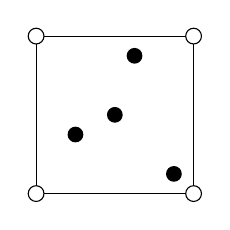
\begin{tikzpicture}
                \draw (0,0) rectangle (2,2);
                \fill[white] (0,0) circle (0.1); \fill[white] (0,2) circle (0.1); \fill[white] (2,0) circle (0.1); \fill[white] (2,2) circle (0.1);
                \draw (0,0) circle (0.1); \draw (0,2) circle (0.1); \draw (2,0) circle (0.1); \draw (2,2) circle (0.1);
                \fill[black] (0.5,0.75) circle (0.1); \fill[black] (1.25,1.75) circle (0.1); \fill[black] (1.75,0.25) circle (0.1); \fill[black] (1,1) circle (0.1);
              \end{tikzpicture}
            \end{column}
            \begin{column}{0.6\textwidth}
              States of particles known at time $t^n$:
              \begin{equation*}
                \left\lbrace\begin{aligned}
                    & \vect{v}^{p,n},\tens{F}^{p,n},\tens{\Pi}^{p,n} \: \rightarrow \:\Ucb^{p,n},\Qcb^{p,n}\\
                    & \vect{X}^{p,n} \: \rightarrow \:M_i^{L,n},K_{ij}^{\alpha,n}
                  \end{aligned}\right.
              \end{equation*}
              
            \end{column}
          \end{columns}
        \end{block}
      \end{column}
    \end{columns}
  \end{footnotesize}
\end{frame}

\begin{frame}{Procedure between $t^n$ and $t^n + \Delta t^n=t^{n+1}$}
  \begin{footnotesize}
    %% Particles -> Nodes
    \begin{equation*}
      \text{Discrete system: }M^L_{i} \frac{\bar{\Ucb}^{i,n+1} - \alert{\bar{\Ucb}^{i,n}}}{\Delta t^n}  - K_{ij}^\alpha \bar{\Fcb}^{j,n}_{\alpha}  + \hat{\Fcb}^{i,n}=  \vect{0}
    \end{equation*}
    \begin{columns}
      \begin{column}{0.4\textwidth}
        \begin{itemize}
        \item[(1)] Computation of matrices $M_i^L$ and $K_{ij}^\alpha$
        \item[(2)] Projection particles $\rightarrow$ nodes
        \end{itemize}
      \end{column}
      \vrule{}
      \begin{column}{0.6\textwidth}
        \begin{block}{Projection particles $\rightarrow$ nodes}
          \begin{columns}
            \begin{column}{0.3\textwidth}
              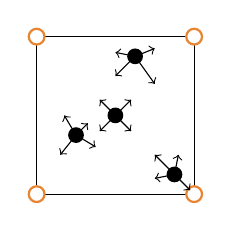
\begin{tikzpicture}
                \draw (0,0) rectangle (2,2);
                \fill[white] (0,0) circle (0.1); \fill[white] (0,2) circle (0.1); \fill[white] (2,0) circle (0.1); \fill[white] (2,2) circle (0.1);
                \draw[Orange,thick] (0,0) circle (0.1); \draw[Orange,thick] (0,2) circle (0.1); \draw[Orange,thick] (2,0) circle (0.1); \draw[Orange,thick] (2,2) circle (0.1);
                \fill[black] (0.5,0.75) circle (0.1); \fill[black] (1.25,1.75) circle (0.1); \fill[black] (1.75,0.25) circle (0.1); \fill[black] (1,1) circle (0.1);
                %% North arrows
                \draw[->,black] (1.25,1.75) -- (1.5,1.85);\draw[->,black] (1.25,1.75) -- (1.,1.8);\draw[->,black] (1.25,1.75) -- (1.,1.5);\draw[->,black] (1.25,1.75) -- (1.5,1.4);
                %% West arrows
                \draw[->,black] (0.5,0.75) -- (0.3,0.5);\draw[->,black] (0.5,0.75) -- (0.35,1.);\draw[->,black] (0.5,0.75) -- (0.75,.6);\draw[->,black] (0.5,0.75) -- (.65,0.9);
                %% Center arrows
                \draw[->,black] (1,1) -- (1.2,1.2);\draw[->,black] (1,1) -- (1.2,0.8);\draw[->,black] (1,1) -- (0.8,1.2);\draw[->,black] (1,1) -- (0.8,0.8);
                %% South arrows
                \draw[->,black] (1.75,0.25) -- (1.95,.05);\draw[->,black] (1.75,0.25) -- (1.8,.5);\draw[->,black] (1.75,0.25) -- (1.5,.5);\draw[->,black] (1.75,0.25) -- (1.5,0.2);
              \end{tikzpicture}
            \end{column}
            \begin{column}{0.6\textwidth}
              \begin{equation*}
                \begin{aligned}
                  & M^{L,n}_i \alert{\bar{\Ucb}^{i,n}} = \sum_{p=1}^{N_p} m_p \bar{\Ucb}^{p,n}\\
                  & M^{L,n}_i \alert{\Qcb^{i,n}} = \sum_{p=1}^{N_p} m_p \Qcb^{p,n}
                \end{aligned}
              \end{equation*}
            \end{column}
          \end{columns}
        \end{block}
      \end{column}
    \end{columns}
  \end{footnotesize}
\end{frame}


\begin{frame}{Procedure between $t^n$ and $t^n + \Delta t^n=t^{n+1}$}
  \begin{footnotesize}
    %% Computation of numerical fluxes (volume + intercell)
    \begin{equation*}
      \text{Discrete system: }M^L_{i} \frac{\bar{\Ucb}^{i,n+1} - \bar{\Ucb}^{i,n}}{\Delta t^n}  - K_{ij}^\alpha \alert{\bar{\Fcb}^{j,n}_{\alpha}}  + \alert{\hat{\Fcb}^{i,n}}=  \vect{0}
    \end{equation*}
    \begin{columns}
      \begin{column}{0.4\textwidth}
        \begin{itemize}
        \item[(1)] Computation of matrices $M_i^L$ and $K_{ij}^\alpha$
        \item[(2)] Projection particles $\rightarrow$ nodes
        \item[(3)] Computation of fluxes
        \end{itemize}
      \end{column}
      \vrule{}
      \begin{column}{0.6\textwidth}
        \begin{block}{Computation of fluxes}
          \begin{columns}
            \begin{column}{0.4\textwidth}
              \begin{block}{\footnotesize Volume fluxes}
                $\bar{\Ucb}^{i,n},\Qcb^{i,n} \rightarrow \bar{\Fcb}^{i,n}_\alpha$
              \end{block}
            \end{column}
            \begin{column}{0.55\textwidth}
              \begin{block}{\footnotesize Intercell fluxes}
                Approximate Riemann solver $\rightarrow \hat{\Fcb}^i$
              \end{block}
            \end{column}
          \end{columns}
        \end{block}
      \end{column}
    \end{columns}
  \end{footnotesize}
\end{frame}

\begin{frame}{Procedure between $t^n$ and $t^n + \Delta t^n=t^{n+1}$}
  \begin{footnotesize}
    %% Time integration 
    \begin{equation*}
      \text{Discrete system: }M^L_{i} \frac{\alert{\bar{\Ucb}^{i,n+1}} - \bar{\Ucb}^{i,n}}{\Delta t^n}  - K_{ij}^\alpha \bar{\Fcb}^{j,n}_{\alpha}  + \hat{\Fcb}^{i,n}=  \vect{0}
    \end{equation*}
    \begin{columns}
      \begin{column}{0.4\textwidth}
        \begin{itemize}
        \item[(1)] Computation of matrices $M_i^L$ and $K_{ij}^\alpha$
        \item[(2)] Projection particles $\rightarrow$ nodes
        \item[(3)] Computation of fluxes
        \item[(4)] Explicit time integration
        \end{itemize}
      \end{column}
      \vrule{}
      \begin{column}{0.6\textwidth}
        \begin{block}{Explicit time integration}
          
          % \begin{columns}
          %   \begin{column}{0.4\textwidth}
              % \begin{tikzpicture}
              %   \draw (0,0) rectangle (2,2);
              %   \fill[white] (0,0) circle (0.1); \fill[white] (0,2) circle (0.1); \fill[white] (2,0) circle (0.1); \fill[white] (2,2) circle (0.1);
              %   \draw (0,0) circle (0.1); \draw (0,2) circle (0.1); \draw (2,0) circle (0.1); \draw (2,2) circle (0.1);
              %   \draw[->,thick] (0,0) -- (0.15,0.15);
              %   \draw[->,thick] (2,0) -- (1.85,0.15);
              %   \draw[->,thick] (2,2) -- (1.85,1.85);
              %   \draw[->,thick] (0,2) -- (.15,1.85);
                
              %   \fill[Orange] (0.5,0.75) circle (0.1); \fill[Orange] (1.25,1.75) circle (0.1); \fill[Orange] (1.75,0.25) circle (0.1); \fill[Orange] (1,1) circle (0.1);
              % \end{tikzpicture}
            % \end{column}
          %   \begin{column}{0.55\textwidth}
          %     \begin{equation*}
          %       \alert{\bar{\Ucb}^{p,n+1}}=\sum_{i=1}^{N_{nodes}} S_{i}(\vect{X}^{p}) \bar{\Ucb}^{i,n+1}
          %     \end{equation*}
          %   \end{column}
          % \end{columns}
        \end{block}
      \end{column}
    \end{columns}
  \end{footnotesize}
\end{frame}

\begin{frame}{Procedure between $t^n$ and $t^n + \Delta t^n=t^{n+1}$}
  \begin{footnotesize}
    %% Interpolation
    \begin{columns}
      \begin{column}{0.4\textwidth}
        \begin{itemize}
        \item[(1)] Computation of matrices $M_i^L$ and $K_{ij}^\alpha$
        \item[(2)] Projection particles $\rightarrow$ nodes
        \item[(3)] Computation of fluxes
        \item[(4)] Explicit time integration
        \item[(5)] Projection nodes $\rightarrow$ particles 
        \end{itemize}
      \end{column}
      \vrule{}
      \begin{column}{0.6\textwidth}
        \begin{block}{Projection nodes $\rightarrow$ particles}
          
          \begin{columns}
            \begin{column}{0.4\textwidth}
              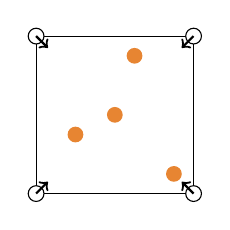
\begin{tikzpicture}
                \draw (0,0) rectangle (2,2);
                \fill[white] (0,0) circle (0.1); \fill[white] (0,2) circle (0.1); \fill[white] (2,0) circle (0.1); \fill[white] (2,2) circle (0.1);
                \draw (0,0) circle (0.1); \draw (0,2) circle (0.1); \draw (2,0) circle (0.1); \draw (2,2) circle (0.1);
                \draw[->,thick] (0,0) -- (0.15,0.15);
                \draw[->,thick] (2,0) -- (1.85,0.15);
                \draw[->,thick] (2,2) -- (1.85,1.85);
                \draw[->,thick] (0,2) -- (.15,1.85);
                
                \fill[Orange] (0.5,0.75) circle (0.1); \fill[Orange] (1.25,1.75) circle (0.1); \fill[Orange] (1.75,0.25) circle (0.1); \fill[Orange] (1,1) circle (0.1);
              \end{tikzpicture}
            \end{column}
            \begin{column}{0.55\textwidth}
              \begin{equation*}
                \alert{\bar{\Ucb}^{p,n+1}}=\sum_{i=1}^{N_{nodes}} S_{i}(\vect{X}^{p}) \bar{\Ucb}^{i,n+1}
              \end{equation*}
            \end{column}
          \end{columns}
        \end{block}
      \end{column}
    \end{columns}
  \end{footnotesize}
\end{frame}

\begin{frame}{Procedure between $t^n$ and $t^n + \Delta t^n=t^{n+1}$}
  \begin{footnotesize}
    %% Kinematic and constitutive updates
    \begin{columns}
      \begin{column}{0.4\textwidth}
        \begin{itemize}
        \item[(1)] Computation of matrices $M_i^L$ and $K_{ij}^\alpha$
        \item[(2)] Projection particles $\rightarrow$ nodes
        \item[(3)] Computation of fluxes
        \item[(4)] Explicit time integration
        \item[(5)] Projection nodes $\rightarrow$ particles 
        \item[(6)] Kinematics and constitutive updates
        \end{itemize}
      \end{column}
      \vrule{}
      \begin{column}{0.6\textwidth}
        \begin{block}{Kinematics and constitutive updates}
          \begin{columns}
            \begin{column}{0.4\textwidth}
              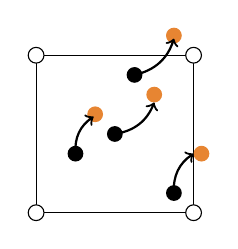
\begin{tikzpicture}
                \draw (0,0) rectangle (2,2);
                \fill[white] (0,0) circle (0.1); \fill[white] (0,2) circle (0.1); \fill[white] (2,0) circle (0.1); \fill[white] (2,2) circle (0.1);
                \draw (0,0) circle (0.1); \draw (0,2) circle (0.1); \draw (2,0) circle (0.1); \draw (2,2) circle (0.1);
                \fill[black] (0.5,0.75) circle (0.1); \fill[black] (1.25,1.75) circle (0.1); \fill[black] (1.75,0.25) circle (0.1); \fill[black] (1,1) circle (0.1);
                \fill[Orange] (0.75,1.25) circle (0.1); \fill[Orange] (1.75,2.25) circle (0.1); \fill[Orange] (2.1,0.75) circle (0.1); \fill[Orange] (1.5,1.5) circle (0.1);
                \path[->,thick,black] (0.5,0.75) edge[bend left] (0.73,1.22);
                \path[->,thick,black] (1.25,1.75) edge[bend right] (1.75,2.21);
                \path[->,thick,black](1.75,0.25) edge[bend left] (2.,0.75);
                \path[->,thick,black](1,1) edge[bend right] (1.5,1.4);
              \end{tikzpicture}
            \end{column}
            \begin{column}{0.55\textwidth}
              \begin{flalign*}
                \begin{aligned}
                  & \alert{\tens{\Pi}^{p,n+1}}=g(\tens{F}^{p,n+1})\\
                  & \alert{\vect{\varphi}^{p,n+1}}= \vect{\varphi}^{p,n} +\Delta t^n \vect{v}^{p,n+1}
                \end{aligned}
              \end{flalign*}
            \end{column}
          \end{columns}
        \end{block}
      \end{column}
    \end{columns}
  \end{footnotesize}
\end{frame}
      
\begin{frame}{Procedure between $t^n$ and $t^n + \Delta t^n=t^{n+1}$}
  \begin{footnotesize}
    %% Rebuild the grid if needed
    \begin{columns}
      \begin{column}{0.4\textwidth}
        \begin{itemize}
        \item[(1)] Computation of matrices $M_i^L$ and $K_{ij}^\alpha$
        \item[(2)] Projection particles $\rightarrow$ nodes
        \item[(3)] Computation of fluxes
        \item[(4)] Explicit time integration
        \item[(5)] Projection nodes $\rightarrow$ particles 
        \item[(6)] Kinematics and constitutive updates
        \item[(7)] Reconstruction of the grid (if needed) 
        \end{itemize}
      \end{column}
      \vrule{}
      \begin{column}{0.6\textwidth}
        \begin{block}{Reconstruction of the grid (if needed)}
          \begin{columns}
            \begin{column}{0.4\textwidth}
              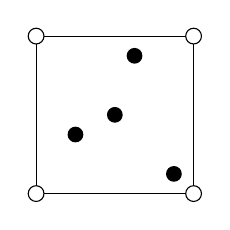
\begin{tikzpicture}
                \draw (0,0) rectangle (2,2);
                \fill[white] (0,0) circle (0.1); \fill[white] (0,2) circle (0.1); \fill[white] (2,0) circle (0.1); \fill[white] (2,2) circle (0.1);
                \draw (0,0) circle (0.1); \draw (0,2) circle (0.1); \draw (2,0) circle (0.1); \draw (2,2) circle (0.1);
                \fill[black] (0.5,0.75) circle (0.1); \fill[black] (1.25,1.75) circle (0.1); \fill[black] (1.75,0.25) circle (0.1); \fill[black] (1,1) circle (0.1);
              \end{tikzpicture}
            \end{column}
            \begin{column}{0.55\textwidth}
              \centering
              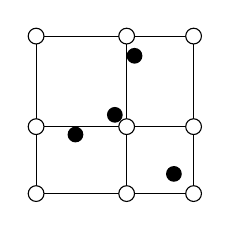
\begin{tikzpicture}
                \draw (0,0) rectangle (2.,2.);
                \draw (1.15,0.85) rectangle (2.,0);
                \draw (1.15,0.85) rectangle (2.,2);
                \draw (1.15,0.85) rectangle (0.,2);
                %% Old nodes
                \fill[white] (0,0) circle (0.1);
                \fill[white] (0,2) circle (0.1);
                \fill[white] (2,0) circle (0.1);
                \fill[white] (2,2) circle (0.1);
                \draw (0,0) circle (0.1);
                \draw (0,2) circle (0.1);
                \draw (2,0) circle (0.1);
                \draw (2,2) circle (0.1);
                
                %% Added nodes
                \fill[white] (1.15,0.85) circle (0.1);
                \fill[white] (0,0.85) circle (0.1);
                \fill[white] (2,0.85) circle (0.1);
                \fill[white] (1.15,0) circle (0.1);
                \fill[white] (1.15,2) circle (0.1);
                \draw (1.15,0.85) circle (0.1);
                \draw (0,0.85) circle (0.1);
                \draw (2,0.85) circle (0.1);
                \draw (1.15,0) circle (0.1);
                \draw (1.15,2) circle (0.1);
                
                %% Particles
                \fill[black] (0.5,0.75) circle (0.1); \fill[black] (1.25,1.75) circle (0.1); \fill[black] (1.75,0.25) circle (0.1); \fill[black] (1,1) circle (0.1);
              \end{tikzpicture}
            \end{column}
          \end{columns}
        \end{block}
      \end{column}
    \end{columns}
  \end{footnotesize}
\end{frame}
%%% Local Variables:
%%% mode: latex
%%% TeX-master: "../presentation"
%%% End:



\subsection{Stability analysis}
\begin{frame}{Linear advection equation of an arbitrary quantity $q$}%{One-dimensional problems}
  \begin{block}{Scheme equation (finite difference sense)}
    \begin{footnotesize}
      \begin{equation*}
        \bar{q}^{p,n+1}=\sum_{k=1}^{N_p}H_{pk}(\vect{X}^p,\vect{X}^k,\text{CFL})\bar{q}^{k,n}
      \end{equation*}
    \end{footnotesize}
  \end{block}
  \begin{block}{von-Neumann linear stability analysis}
    \begin{footnotesize}
      The numerical scheme is stable if:
      \begin{equation*}
        \sum_{k=1}^{N_p}\abs{H_{pk}} \leq 1 \quad \forall p
      \end{equation*}
      \alert{$\Rightarrow$ find the maximal CFL number ensuring the stability}
    \end{footnotesize}
  \end{block}\pause
  \metroset{block=fill}
  \begin{footnotesize}
    \begin{block}{Particular case: one particle per cell}
      The \textbf{first-order} FVM is recovered $\rightarrow$ CFL improved compared to MPM and DGFEM
    \end{block}
  \end{footnotesize}
\end{frame}


%%% Local Variables:
%%% mode: latex
%%% TeX-master: "../presentation"
%%% End:



\section{Numerical simulations}

\subsection{Linearized geometrical framework}
\begin{frame}{\href{section4/animation/elasticity_stress/video.mp4}{Plane strain elasticity}}
  \begin{overprint}
    \onslide<1>
    \vspace{-1.cm}
    \begin{columns}
      \begin{column}{0.42\linewidth}
        \input{section4/pgfFigures/2d_square}
      \end{column}

      \begin{column}{0.6\linewidth}
        \vspace{1.5cm}
        \centering
        \phantom{\begin{tikzpicture}
  \begin{groupplot}[group style={group size=2 by 1,
ylabels at=edge left, yticklabels at=edge left,horizontal sep=1.5ex,
xticklabels at=edge bottom,xlabels at=edge bottom},
ymajorgrids=true,xmajorgrids=true,xlabel=$x \: (m)$,
axis on top,scale only axis,width=0.43\linewidth, every x tick scale label/.style={at={(xticklabel* cs:1.05,0.75cm)},anchor=near yticklabel},ymin=-0.5e6,ymax=.5e9,xmin=0,xmax=3]
\nextgroupplot[ylabel=$\sigma_{11}\: (Pa)$,title={$t=2.5 \times 10^{-4} \: s$},every y tick scale label/.style={at={(-0.,1.1)}}]
\addplot[Red,very thick,no markers] table[x=Points:0,y=S11] {section4/csvFiles/2delast_fem_115.csv};

\addplot[Blue,very thick,mark=+,only marks,mark size=3pt] table[x=Points:0,y=stress_11] {section4/csvFiles/2delast_ctu1ppc_115.csv};
\addplot[Purple,very thick,mark=asterisk,only marks,mark size=2pt] table[x=Points:0,y=stress_11] {section4/csvFiles/2delast_ctu4ppc_115.csv};
\addplot[Orange,very thick,mark=x,only marks,mark size=3pt] table[x=Points:0,y=mpm_S11] {section4/csvFiles/2delast_mpm_115.csv};

\nextgroupplot[legend style={at={($(0.22,-0.3)+(1.cm,0cm)$)},legend columns=2},xlabel=$x (m)$,title={$t=1.0 \times 10^{-3} \: s$},ytick scale label code/.code={}]
\addplot[Red,very thick,no markers] table[x=Points:0,y=S11] {section4/csvFiles/2delast_fem_338.csv};
\addplot[Blue,very thick,mark=+,only marks,mark size=3pt] table[x=Points:0,y=stress_11] {section4/csvFiles/2delast_ctu1ppc_338.csv};
\addplot[Purple,very thick,mark=asterisk,only marks,mark size=2pt] table[x=Points:0,y=stress_11] {section4/csvFiles/2delast_ctu4ppc_338.csv};
\addplot[Orange,very thick,mark=x,only marks,mark size=3pt] table[x=Points:0,y=mpm_S11] {section4/csvFiles/2delast_mpm_338.csv};
\addlegendentry{fem}
\addlegendentry{ctu 1ppc}
\addlegendentry{ctu 4ppc}
\addlegendentry{mpm}
   
  \end{groupplot}
\end{tikzpicture}


%%% Local Variables:
%%% mode: latex
%%% TeX-master: "../../aRenaud"
%%% End:




































%%% Local Variables:
%%% mode: latex
%%% TeX-master: "../../mainManuscript"
%%% End:
}
      \end{column}
      
    \end{columns}
    \onslide<2>
    \vspace{-1.cm}
    \begin{columns}
      \begin{column}{0.42\linewidth}
        \movie[height=.7\paperheight,width=1.\linewidth,showcontrols,loop,poster,autostart]{%\input{section4/pgfFigures/2d_square}
        }{section4/animation/elasticity_stress/video.mp4}
      \end{column}

      \begin{column}{0.6\linewidth}
        \vspace{1.5cm}
        \centering
        \begin{tikzpicture}
  \begin{groupplot}[group style={group size=2 by 1,
ylabels at=edge left, yticklabels at=edge left,horizontal sep=1.5ex,
xticklabels at=edge bottom,xlabels at=edge bottom},
ymajorgrids=true,xmajorgrids=true,xlabel=$x \: (m)$,
axis on top,scale only axis,width=0.43\linewidth, every x tick scale label/.style={at={(xticklabel* cs:1.05,0.75cm)},anchor=near yticklabel},ymin=-0.5e6,ymax=.5e9,xmin=0,xmax=3]
\nextgroupplot[ylabel=$\sigma_{11}\: (Pa)$,title={$t=2.5 \times 10^{-4} \: s$},every y tick scale label/.style={at={(-0.,1.1)}}]
\addplot[Red,very thick,no markers] table[x=Points:0,y=S11] {section4/csvFiles/2delast_fem_115.csv};

\addplot[Blue,very thick,mark=+,only marks,mark size=3pt] table[x=Points:0,y=stress_11] {section4/csvFiles/2delast_ctu1ppc_115.csv};
\addplot[Purple,very thick,mark=asterisk,only marks,mark size=2pt] table[x=Points:0,y=stress_11] {section4/csvFiles/2delast_ctu4ppc_115.csv};
\addplot[Orange,very thick,mark=x,only marks,mark size=3pt] table[x=Points:0,y=mpm_S11] {section4/csvFiles/2delast_mpm_115.csv};

\nextgroupplot[legend style={at={($(0.22,-0.3)+(1.cm,0cm)$)},legend columns=2},xlabel=$x (m)$,title={$t=1.0 \times 10^{-3} \: s$},ytick scale label code/.code={}]
\addplot[Red,very thick,no markers] table[x=Points:0,y=S11] {section4/csvFiles/2delast_fem_338.csv};
\addplot[Blue,very thick,mark=+,only marks,mark size=3pt] table[x=Points:0,y=stress_11] {section4/csvFiles/2delast_ctu1ppc_338.csv};
\addplot[Purple,very thick,mark=asterisk,only marks,mark size=2pt] table[x=Points:0,y=stress_11] {section4/csvFiles/2delast_ctu4ppc_338.csv};
\addplot[Orange,very thick,mark=x,only marks,mark size=3pt] table[x=Points:0,y=mpm_S11] {section4/csvFiles/2delast_mpm_338.csv};
\addlegendentry{fem}
\addlegendentry{ctu 1ppc}
\addlegendentry{ctu 4ppc}
\addlegendentry{mpm}
   
  \end{groupplot}
\end{tikzpicture}


%%% Local Variables:
%%% mode: latex
%%% TeX-master: "../../aRenaud"
%%% End:




































%%% Local Variables:
%%% mode: latex
%%% TeX-master: "../../mainManuscript"
%%% End:

      \end{column}
    \end{columns}
  \end{overprint}
\end{frame}


\begin{frame}{Plane strain elastoplasticity}
  \begin{overprint}
    \onslide<1>
    \vspace{0.25cm}
    \centering
    \movie[height=.7\paperheight,width=.75\linewidth,showcontrols,loop,poster,autostart]{
    }{section4/animation/elastoplasticity/video.ogv}
    \onslide<2>
    \centering
    \begin{tikzpicture}[scale=0.49]
  \begin{groupplot}[group style={group size=1 by 2,
ylabels at=edge left, yticklabels at=edge left,horizontal sep=3.ex,vertical sep=4.ex,
xticklabels at=edge bottom,xlabels at=edge bottom},
ymajorgrids=true,xmajorgrids=true,
axis on top,scale only axis, every x tick scale label/.style={at={(xticklabel* cs:1.05,0.75cm)},anchor=near yticklabel}]
\nextgroupplot[ylabel=\normalsize $\sigma_{11}$ (Pa)]
\addplot[Red,very thick,no markers] table[x=Points:0,y=S11] {appendix/csvFiles/2dEP_fem_115.csv};
\addplot[Blue,very thick,mark=+,only marks,mark size=3pt] table[x=Points:0,y=stress_11] {appendix/csvFiles/2dEP_ctu1ppc_115.csv};
\addplot[Purple,very thick,mark=square,only marks] table[x=Points:0,y=stress_11] {appendix/csvFiles/2dEP_ctu4ppc_115.csv};
\addplot[Orange,very thick,mark=x,only marks,mark size=3pt] table[x=Points:0,y= mpm_S11] {appendix/csvFiles/2dEP_mpm_115.csv};

% \nextgroupplot[title={(b) $t=1.0 \times 10^{-3} \: s$},ymin=-0.5e6,ymax=1.5e9]
% \addplot[Red,very thick,no markers] table[x=Points:0,y=S11] {appendix/csvFiles/2dEP_fem_338.csv};
% \addplot[Blue,very thick,mark=+,only marks,mark size=3pt] table[x=Points:0,y=stress_11] {appendix/csvFiles/2dEP_ctu1ppc_338.csv};
% \addplot[Purple,very thick,mark=square,only marks] table[x=Points:0,y=stress_11] {appendix/csvFiles/2dEP_ctu4ppc_338.csv};
% \addplot[Orange,very thick,mark=x,only marks,mark size=3pt] table[x=Points:0,y= mpm_S11] {appendix/csvFiles/2dEP_mpm_338.csv};

\nextgroupplot[%legend style={at={($(0.12,-0.35)+(5cm,5cm)$)},legend columns=1}
legend pos={north east},
,ylabel=\normalsize $\eps^p_{11}$,xlabel=\normalsize $x$ (m)]
\addplot[Red,very thick,no markers] table[x=Points:0,y=EP11] {appendix/csvFiles/2dEP_fem_115.csv};
\addplot[Blue,very thick,mark=+,only marks,mark size=3pt] table[x=Points:0,y=epsp_11] {appendix/csvFiles/2dEP_ctu1ppc_115.csv};
\addplot[Purple,very thick,mark=square,only marks] table[x=Points:0,y=epsp_11] {appendix/csvFiles/2dEP_ctu4ppc_115.csv};
\addplot[Orange,very thick,mark=x,only marks,mark size=3pt] table[x=Points:0,y= mpm_epsp11] {appendix/csvFiles/2dEP_mpm_115.csv};

% \nextgroupplot[legend style={at={($(0.12,-0.35)+(0.9cm,1cm)$)},legend columns=2},xlabel=$x (m)$,ymin=-0.1e-3,ymax=6.75e-3]
% \addplot[Red,very thick,no markers] table[x=Points:0,y=EP11] {appendix/csvFiles/2dEP_fem_338.csv};
% \addplot[Blue,very thick,mark=+,only marks,mark size=3pt] table[x=Points:0,y=epsp_11] {appendix/csvFiles/2dEP_ctu1ppc_338.csv};
% \addplot[Purple,very thick,mark=square,only marks] table[x=Points:0,y=epsp_11] {appendix/csvFiles/2dEP_ctu4ppc_338.csv};
% \addplot[Orange,very thick,mark=x,only marks,mark size=3pt] table[x=Points:0,y= mpm_epsp11] {appendix/csvFiles/2dEP_mpm_338.csv};
\addlegendentry{fem}
\addlegendentry{ctu 1ppc}
\addlegendentry{ctu 4ppc}
\addlegendentry{mpm}
   
  \end{groupplot}
\end{tikzpicture}


%%% Local Variables:
%%% mode: latex
%%% TeX-master: "../../presentation"
%%% End:




































%%% Local Variables:
%%% mode: latex
%%% TeX-master: "../../presentation"
%%% End:

  \end{overprint}

\end{frame}
%%% Local Variables:
%%% mode: latex
%%% TeX-master: "../aRenaud"
%%% End:
\subsection{Large strains framework}
% \begin{frame}
% \begin{tikzpicture}[remember picture,overlay]
%   \node[anchor=south west, inner sep=0pt] at (current page.south west) {%
%     \includemedia[
%     addresource=section4/animation/hyperelasticity_velo/video.mp4,
%     activate=pageopen,transparent,
%     flashvars={source=section4/animation/hyperelasticity_velo/video.mp4},
%     width=\paperwidth,height=\paperheight
%     ]{}{VPlayer.swf}%
%   };
% \end{tikzpicture}
% \end{frame}

\begin{frame}%{\href{section4/animation/hyperelasticity_velo/video.mp4}{2D hyperelasticity}}
  \begin{center}
    % \movie[width=1.\linewidth,showcontrols,loop]{\input{section4/pgfFigures/2d_square}}{section4/animation/hyperelasticity_velo/video.mp4}
    \href{section4/animation/hyperelasticity_velo/video.mp4}{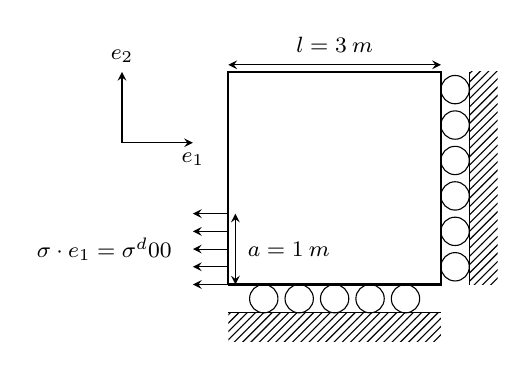
\begin{tikzpicture}[scale=0.9]
  \draw[thick] (0,0) --(3,0)--(3,3)--(0,3)--(0,0);
  \foreach \x in {0.5,1.,...,2.5} 
  \draw(\x,-0.2)circle(0.2);
  \foreach \x in {0.25,0.75,...,2.75} 
  \draw(3.2,\x)circle(0.2);
  \draw(0,-0.4)--(3.,-0.4);
  \draw(3.4,0)--(3.4,3);
  \fill [pattern=north east lines](0.0,-0.8)rectangle+(3,0.4);
  \fill [pattern=north east lines](3.4,0.)rectangle+(0.4,3);
  \draw[>=stealth,<->](0,3.1)--node[above=1pt]{\footnotesize $l=3 \: m$}(3,3.1);
  \draw[>=stealth,<->](0.1,0)--node[right=1pt]{\footnotesize $a=1 \: m$}(0.1,1);
  \foreach \x in {0.,0.25,...,1} 
  \draw[>=stealth,<-] (-0.5,\x)--(0.,\x);
  \node(a)at(-1.75,0.5){\footnotesize $\tens{\sigma}\cdot\vect{e}_1=\matrice{\sigma^d\\0 \\0}$}; 
  \draw[>=stealth,->](-1.5,2)--(-0.5,2)node(a)[anchor=north]{\footnotesize $\vect{e}_1$};
  \draw[>=stealth,->](-1.5,2)--(-1.5,3)node(a)[anchor=south]{\footnotesize $\vect{e}_2$};
\end{tikzpicture}
% \input{section4/pgfFigures/2d_square}
}
    % \movie[height = \paperheight, width = \paperwidth, poster,showcontrols,loop]{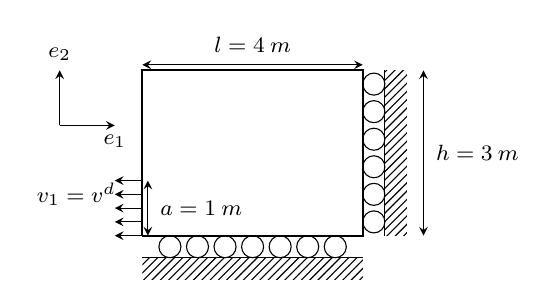
\begin{tikzpicture}[scale=0.7]
  \draw[thick] (0,0) --(4,0)--(4,3)--(0,3)--(0,0);
  \foreach \x in {0.5,1.,...,3.5} 
  \draw(\x,-0.2)circle(0.2);
  \foreach \x in {0.25,0.75,...,2.75} 
  \draw(4.2,\x)circle(0.2);
  \draw(0,-0.4)--(4.,-0.4);
  \draw(4.4,0)--(4.4,3);
  \fill [pattern=north east lines](0.0,-0.8)rectangle+(4,0.4);
  \fill [pattern=north east lines](4.4,0.)rectangle+(0.4,3);
  \draw[>=stealth,<->](5.1,0)--node[right=1pt]{\footnotesize $h=3 \: m$}(5.1,3);
  \draw[>=stealth,<->](0,3.1)--node[above=1pt]{\footnotesize $l=4 \: m$}(4,3.1);
  \draw[>=stealth,<->](0.1,0)--node[right=1pt]{\footnotesize $a=1 \: m$}(0.1,1);
  \foreach \x in {0.,0.25,...,1} 
  \draw[>=stealth,<-] (-0.5,\x)--(0.,\x);
  \node(a)at(-1.2,0.75){\footnotesize $v_1=v^d$}; 
  \draw[>=stealth,->](-1.5,2)--(-0.5,2)node(a)[anchor=north]{\footnotesize $\vect{e}_1$};
  \draw[>=stealth,->](-1.5,2)--(-1.5,3)node(a)[anchor=south]{\footnotesize $\vect{e}_2$};
\end{tikzpicture}

%%% Local Variables:
%%% mode: latex
%%% TeX-master: "../../mainManuscript"
%%% End:}{section4/animation/hyperelasticity_velo/video.mp4}
    % \animategraphics[loop,controls,width=1.\linewidth,autoplay]{10}{animation/hyperelasticity_velo/animation-}{0}{3}
  \end{center}
\end{frame}


%%% Local Variables:
%%% mode: latex
%%% TeX-master: "../aRenaud"
%%% End:




%%% Local Variables:
%%% mode: latex
%%% TeX-master: "../aRenaud"
%%% End:




\section{Elastoplastic hyperbolic problems in two space dimensions}


\subsection{Historical review}
%% Problèmes traités -- approche expérimentale pour la confirmation
%% Type de solutions
%% Simple waves even for linear hardening in contrast to one-dimensional problems

\begin{frame}{Thin-walled tube problem}%{Historical review}
  %% References: Lin_et_Ballman,Li_planeStress_EP,Wu_experimental,Ting73,Clifton_exp2,Valanis,Clifton_exp,Ting69,Bleich,Clifton,CRISTESCU19591605,Rakhmatulin
  \begin{overprint}
    \onslide<1>
    \begin{columns}
      \begin{column}{0.4\textwidth}
        \begin{block}{\footnotesize Semi-infinite medium}
          % \centering
          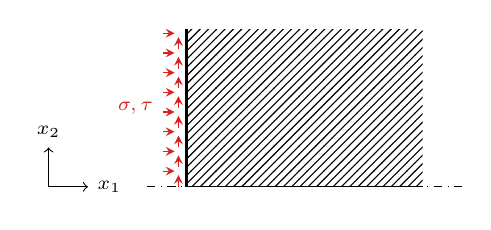
\begin{tikzpicture}
            \begin{scope}[shift={(-1.75,0)}]
              \draw[->] (0,0) -- (0.5,0) node[right] {\scriptsize $x_1$};
              \draw[->] (0,0) -- (0,0.5) node[above] {\scriptsize $x_2$};
            \end{scope}
            \draw (0,0) -- (3,.0);
            \draw[very thick] (0,0) -- (0,2.);
            \fill [pattern=north east lines] (0,0) rectangle (3.,2.);
            \draw[dash dot] (-0.5,0) -- (3.5,0);% node[right] {\footnotesize $x_1$};
            % \draw[->,dash dot] (0,0) -- (0,2.5) node[above] {\footnotesize $x_2$};
            \foreach \y in {0,0.25,...,1.75}
            \draw[Red,->,>=stealth] (-0.1,\y) -- (-0.1,\y+0.15);
            \foreach \y in {0,0.25,...,1.75}
            \draw[Red,->,>=stealth] (-0.30,\y+0.20) -- (-0.15,\y+0.20);
            \node[Red,left] at (-0.3,1.) {\scriptsize $\sigma,\tau$};
          \end{tikzpicture}  
        \end{block}
      \end{column}
      \begin{column}{0.62\textwidth}
        \begin{footnotesize}
          \begin{block}{\footnotesize Elastic solution}
            \begin{columns}
              \begin{column}{0.35\textwidth}
                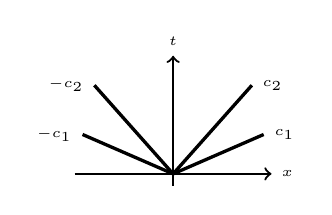
\begin{tikzpicture}[scale=0.5]
                  \draw[thick,->] (-2.5,0) -- (2.5,0) node[right] {\tiny $x$};
                  \draw[thick,->] (-0.,-0.3) -- (0,3) node[above] {\tiny $t$};
                  \draw[very thick] (0,0) -- (2.3,1.) node[right] {\tiny $c_1$};
                  \draw[very thick] (0,0) -- (-2.3,1.) node[left] {\tiny $-c_1$};
                  \draw[very thick] (0,0) -- (2.,2.25) node[right] {\tiny $c_2$};
                  \draw[very thick] (0,0) -- (-2.,2.25) node[left] {\tiny $-c_2$};
                \end{tikzpicture}
              \end{column}
              \begin{column}{0.6\textwidth}
                \begin{itemize}
                \item[] pressure and shear waves: $c_1,c_2$
                \item[] discontinuous waves
                \end{itemize}
              \end{column}
            \end{columns}
          \end{block}
        \end{footnotesize}
      \end{column}
    \end{columns}
    \onslide<2>
    \begin{columns}
      \begin{column}{0.4\textwidth}
        \begin{block}{\footnotesize Semi-infinite medium}
          % \centering
          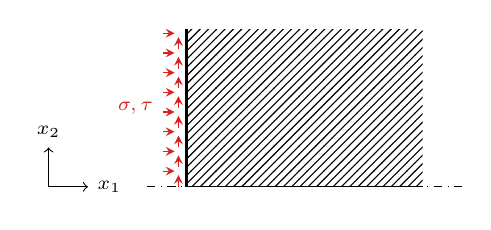
\begin{tikzpicture}
            \begin{scope}[shift={(-1.75,0)}]
              \draw[->] (0,0) -- (0.5,0) node[right] {\scriptsize $x_1$};
              \draw[->] (0,0) -- (0,0.5) node[above] {\scriptsize $x_2$};
            \end{scope}
            \draw (0,0) -- (3,.0);
            \draw[very thick] (0,0) -- (0,2.);
            \fill [pattern=north east lines] (0,0) rectangle (3.,2.);
            \draw[dash dot] (-0.5,0) -- (3.5,0);% node[right] {\footnotesize $x_1$};
            % \draw[->,dash dot] (0,0) -- (0,2.5) node[above] {\footnotesize $x_2$};
            \foreach \y in {0,0.25,...,1.75}
            \draw[Red,->,>=stealth] (-0.1,\y) -- (-0.1,\y+0.15);
            \foreach \y in {0,0.25,...,1.75}
            \draw[Red,->,>=stealth] (-0.30,\y+0.20) -- (-0.15,\y+0.20);
            \node[Red,left] at (-0.3,1.) {\scriptsize $\sigma,\tau$};
          \end{tikzpicture}  
        \end{block}
      \end{column}
      \begin{column}{0.62\textwidth}
        \begin{footnotesize}
          \begin{block}{\footnotesize Elastic-\alert{plastic} solution \cite{CRISTESCU19591605,Rakhmatulin}}
            \begin{columns}
              \begin{column}{0.35\textwidth}
                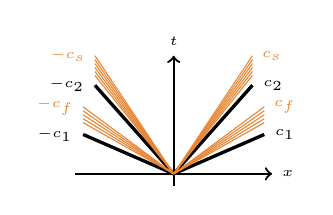
\begin{tikzpicture}[scale=0.5]
                  \draw[thick,->] (-2.5,0) -- (2.5,0) node[right] {\tiny $x$};
                  \draw[thick,->] (-0.,-0.3) -- (0,3) node[above] {\tiny $t$};
                  \draw[very thick] (0,0) -- (2.3,1.) node[right] {\tiny $c_1$};
                  \draw[very thick] (0,0) -- (-2.3,1.) node[left] {\tiny $-c_1$};
                  \draw[very thick] (0,0) -- (2.,2.25) node[right] {\tiny $c_2$};
                  \draw[very thick] (0,0) -- (-2.,2.25) node[left] {\tiny $-c_2$};
                  \foreach \x in {1.3,1.4,1.5,1.6,1.7}
                  {\draw[Orange] (0,0)-- (2.3,\x);
                    \draw[Orange] (0,0)-- (-2.3,\x);}
                  \node[Orange,right] at (2.3,1.7) {\tiny $c_f$};
                  \node[Orange,left] at (-2.3,1.7) {\tiny $-c_f$};
                  \foreach \x in {2.5,2.6,2.7,2.8,2.9,3.}
                  {\draw[Orange] (0,0)-- (2,\x);
                    \draw[Orange] (0,0)-- (-2,\x);}
                  \node[Orange,right] at (2,3) {\tiny $c_s$};
                  \node[Orange,left] at (-2,3) {\tiny $-c_s$};
                \end{tikzpicture}
              \end{column}
              \begin{column}{0.6\textwidth}
                \begin{itemize}
                \item[] fast and slow simple waves: $c_f,c_s$
                \item[] combined-stress waves
                \end{itemize}
              \end{column}
            \end{columns}
          \end{block}
        \end{footnotesize}
      \end{column}
    \end{columns}
    \footnoteCite{CRISTESCU19591605,Rakhmatulin}
  \end{overprint}
\end{frame}


\begin{frame}{Thin-walled tube problem}
  %% Détailler travaux de clifton, comment il en arrive à des trajets élémentaires
  %% Problème de Picard
  \begin{block}{Characteristic analysis of the elastic-plastic hyperbolic system \cite{Clifton}}
    \begin{footnotesize}
      \begin{columns}
        \begin{column}{0.6\textwidth}
          \begin{itemize}
            % \item ODEs governing the evolution of stress and velocity through both simple waves
          \item[] ODEs through simple waves: $d\tau=\psi(\tens{\sigma})d\sigma$ 
            \begin{itemize}
            \item \footnotesize integration $\rightarrow$ loading paths
            \item \footnotesize mathematical study $\rightarrow$ solution of Picard's problem
            \end{itemize}
            \centering
            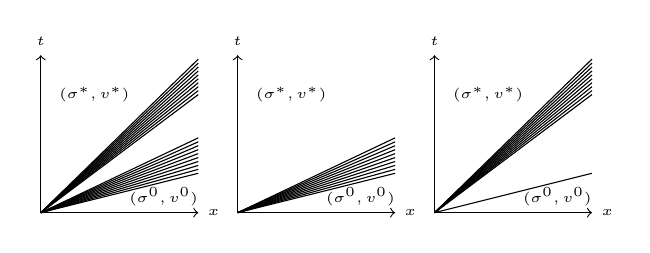
\begin{tikzpicture}
              \draw[->] (0,0) -- (2,0) node[right] {\tiny $x$};
              \draw[->] (0,0) -- (0,2) node[above] {\tiny $t$};
              \node[right] at (1,0.2) {\tiny $(\tens{\sigma}^0,\vect{v}^0)$};
              \draw (0,0) -- (2,0.5);
              \foreach \y in {0.55,0.6,...,1.}
              \draw (0,0) -- (2,\y);
              \foreach \y in {1.5,1.55,...,2.}
              \draw (0,0) -- (2,\y);
              \node[left] at (1.25,1.5) {\tiny $(\tens{\sigma}^*,\vect{v}^*)$};
              \begin{scope}[shift={(2.5,0)}]
                \draw[->] (0,0) -- (2,0) node[right] {\tiny $x$};
                \draw[->] (0,0) -- (0,2) node[above] {\tiny $t$};
                \node[right] at (1,0.2) {\tiny $(\tens{\sigma}^0,\vect{v}^0)$};
                \draw (0,0) -- (2,0.5);
                \foreach \y in {0.55,0.6,...,1.}
                \draw (0,0) -- (2,\y);
                % \foreach \y in {1.5,1.55,...,2.}
                % \draw (0,0) -- (2,\y);
                \node[left] at (1.25,1.5) {\tiny $(\tens{\sigma}^*,\vect{v}^*)$};
              \end{scope}
              \begin{scope}[shift={(5,0)}]
                \draw[->] (0,0) -- (2,0) node[right] {\tiny $x$};
                \draw[->] (0,0) -- (0,2) node[above] {\tiny $t$};
                \node[right] at (1,0.2) {\tiny $(\tens{\sigma}^0,\vect{v}^0)$};
                \draw (0,0) -- (2,0.5);
                \foreach \y in {1.5,1.55,...,2.}
                \draw (0,0) -- (2,\y);
                \node[left] at (1.25,1.5) {\tiny $(\tens{\sigma}^*,\vect{v}^*)$};
              \end{scope}
            \end{tikzpicture}
          %\item confirmed by experimental data \cite{Clifton_exp}
          \end{itemize}
        \end{column}
        \begin{column}{0.43\textwidth}
          \vskip 5pt
          \centering
          \begin{tikzpicture}[scale=0.9]
  \begin{axis}[ymajorgrids=true,xmajorgrids=true,ylabel=$\sigma_{12}$,xlabel=$\sigma_{11}$,xmax=2.e8]
    %%
    \addplot[Green,mark=x,only marks,mark repeat=15,very thick] table [x=sigma_11,y=sigma_12] {chapter5/pgfFigures/pgf_thinWalledTubeSlowWave/slowStressPlane_Stress0.pgf};
    \addplot[Green,thick] table [x=sigma_11,y=sigma_12] {chapter5/pgfFigures/pgf_thinWalledTubeSlowWave/TWslowStressPlane_Stress0.pgf};
    %%
    \addplot[Duck,mark=x,only marks,mark repeat=15,very thick] table [x=sigma_11,y=sigma_12] {chapter5/pgfFigures/pgf_thinWalledTubeSlowWave/slowStressPlane_Stress1.pgf};
    \addplot[Duck,thick] table [x=sigma_11,y=sigma_12] {chapter5/pgfFigures/pgf_thinWalledTubeSlowWave/TWslowStressPlane_Stress1.pgf};
    %%
    \addplot[Red,mark=x,only marks,mark repeat=15,very thick] table [x=sigma_11,y=sigma_12] {chapter5/pgfFigures/pgf_thinWalledTubeSlowWave/slowStressPlane_Stress2.pgf};
    \addplot[Red,thick] table [x=sigma_11,y=sigma_12] {chapter5/pgfFigures/pgf_thinWalledTubeSlowWave/TWslowStressPlane_Stress2.pgf};
    %%
    \addplot[Purple,mark=x,only marks,mark repeat=15,very thick] table [x=sigma_11,y=sigma_12] {chapter5/pgfFigures/pgf_thinWalledTubeSlowWave/slowStressPlane_Stress3.pgf};
    \addplot[Purple,thick] table [x=sigma_11,y=sigma_12] {chapter5/pgfFigures/pgf_thinWalledTubeSlowWave/TWslowStressPlane_Stress3.pgf};
    %%
    \addplot[Blue,mark=x,only marks,mark repeat=15,very thick] table [x=sigma_11,y=sigma_12] {chapter5/pgfFigures/pgf_thinWalledTubeSlowWave/slowStressPlane_Stress4.pgf};
    \addplot[Blue,thick] table [x=sigma_11,y=sigma_12] {chapter5/pgfFigures/pgf_thinWalledTubeSlowWave/TWslowStressPlane_Stress4.pgf};
    %%
    \addplot[Orange,mark=x,only marks,mark repeat=15,very thick] table [x=sigma_11,y=sigma_12] {chapter5/pgfFigures/pgf_thinWalledTubeSlowWave/slowStressPlane_Stress5.pgf};
    \addplot[Orange,thick] table [x=sigma_11,y=sigma_12] {chapter5/pgfFigures/pgf_thinWalledTubeSlowWave/TWslowStressPlane_Stress5.pgf};
    %%
    \addplot[Yellow,mark=x,only marks,mark repeat=5,very thick] table [x=sigma_11,y=sigma_12] {chapter5/pgfFigures/pgf_thinWalledTubeSlowWave/slowStressPlane_Stress6.pgf};
    \addplot[Yellow,thick] table [x=sigma_11,y=sigma_12] {chapter5/pgfFigures/pgf_thinWalledTubeSlowWave/TWslowStressPlane_Stress6.pgf};
    %% Yield surface
    \addplot[black,dashed] table  [x=sigma_11,y=sigma_12] {chapter5/pgfFigures/pgf_thinWalledTubeSlowWave/TWslow_yield0.pgf};
  \end{axis}
\end{tikzpicture}

%%% Local Variables:
%%% mode: latex
%%% TeX-master: "../../mainManuscript"
%%% End:
        \end{column}
      \end{columns}
    \end{footnotesize}
  \end{block}
  % \cite{Clifton,Clifton_exp}
  \footnoteCite{Clifton}
  %% Other problems + difficulties involved + mathematical properties
\end{frame}
\subsection{General formulation}



%%% Local Variables:
%%% mode: latex
%%% TeX-master: "../presentation"
%%% End:





\end{document}

%%% Local Variables:
%%% mode: latex
%%% TeX-master: t
%%% End:
